%% Copyright (C) 2012 Minh Van Nguyen <mvngu.name@gmail.com>
%% This work is licensed under a the GNU Free Documentation License version
%% 1.3.  For the full terms of the license, see
%% http://www.gnu.org/licenses/fdl.html

\documentclass{beamer}

\usepackage{mystyle}


%%%%%%%%%%%%%%%%%%%%%%%%%%%%%%%%%%%%%%%%%%%%%%%%%%%%%%%%%%%%%%%%%%%%%%%%%%%

\title[Evolution of communities]{
  Evolution of communities in \\
  complex networks
}
\institute{
  \large University of Melbourne
}
\author[Minh Van Nguyen]{
  Minh Van Nguyen \\
  \url{mvngu.name@gmail.com}
}
%% uncomment the following line for the current date
\date{\small \today}
%% \date{}


%%%%%%%%%%%%%%%%%%%%%%%%%%%%%%%%%%%%%%%%%%%%%%%%%%%%%%%%%%%%%%%%%%%%%%%%%%%

\begin{document}

\frame{\titlepage}


%%%%%%%%%%%%%%%%%%%%%%%%%%%%%%%%%%%%%%%%%%%%%%%%%%%%%%%%%%%%%%%%%%%%%%%%%%%

\frame{
  \frametitle{Contents}
  \tableofcontents
}


%%%%%%%%%%%%%%%%%%%%%%%%%%%%%%%%%%%%%%%%%%%%%%%%%%%%%%%%%%%%%%%%%%%%%%%%%%%

\section{Why model communities?}
%%
\frame{
  \frametitle{Why model communities?}
  %%
  \begin{itemize}
  \item The presence of communities in social networks is intuitive.
    %% Think of members of a social club such as a sports club, a
    %% professional association such as the ACM, the developers of a
    %% software project, or online communities such as Facebook
    %% groups.  The concept of communities can also be transferred to
    %% other types of networks.  In a financial or economic network, a
    %% community might be a group of organizations that trade more
    %% amongst themselves than with other organizations.  In a
    %% software network, a community might be a group of functions or
    %% modules that invoke each other more often than other functions
    %% or modules in a software package.
  \end{itemize}

  \begin{figure}[!bp]
  \centering
  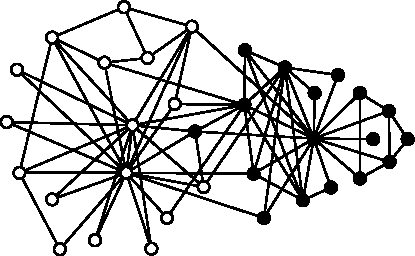
\includegraphics{image/Zachary-karate-club-community}
  \caption{Two communities in a karate club~\cite{Zachary1977}.}
  \end{figure}
}
%%
\frame{
  \frametitle{Why model communities?}
  %%
  \begin{itemize}
  %% By modelling communities over time, we can answer a number of
  %% questions about the life-cycle and evolution of communities found
  %% in online social networks, professional collaboration, and other
  %% types of networks.
  \item For how long is a community typically active?
    %% This question relates to the lifespan of a community.  If a
    %% community comes into existence, one basic question we can ask
    %% is: How long does the community live before it is dead?

  \item Why is it that some communities have more changes throughout
    their lifetimes?
    %% Similarly, why is it that a large number of communities are
    %% more stable throughout their lifetime than other communities?

  \item Which communities are more influential/popular than others?
    %% This question is concerned with identifying communities that
    %% attract many more nodes than other communities.  It is also
    %% about finding out which communities would be efficient for
    %% spreading opinions or epidemics.

  \item Removing which communities would result in the greatest damage
    to a network?
    %% This is a question about the robustness or resilience of
    %% networks.
  \end{itemize}

  \begin{figure}[!bp]
  \centering
  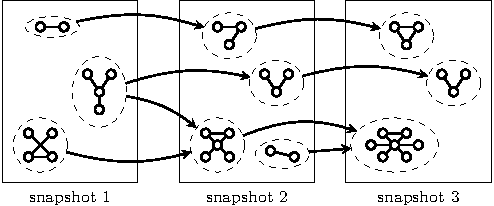
\includegraphics{image/match}
  \caption{}
  \end{figure}
}


%%%%%%%%%%%%%%%%%%%%%%%%%%%%%%%%%%%%%%%%%%%%%%%%%%%%%%%%%%%%%%%%%%%%%%%%%%%

\bibliographystyle{bibliography.bst}
\bibliography{bibliography}

\end{document}
